
\documentclass[a4paper,12pt]{article}
\usepackage{amsmath}
\usepackage{geometry}
\usepackage{graphicx}
\usepackage{subcaption}
\geometry{margin=1in}
\graphicspath{ {Images/} }
\begin{document}


%%%%%%%%%%%%%%%%%%%%%%%%%%%%%%%%%%%%%%%%%%%%%%%%%%%%%%%%%%%%%%%%%%%%%%%%%%%%%%% TITLEPAGE
\pagenumbering{gobble}
\centering
\vspace*{5cm}
{\huge Developing AntBot: \par Visual Navigation based on the insect brain \par}
\vspace{1cm}
{\itshape Robert Mitchell}

\vspace{2cm}

{\large Master of Informatics \par}
{\large Informatics \par}
{\large School of Informatics \par}
{\large The University of Edinburgh \par}
\large \today \par

\vfill
Supervised by\par
Dr. Barbara Webb

\newpage

%%%%%%%%%%%%%%%%%%%%%%%%%%%%%%%%%%%%%%%%%%%%%%%%%%%%%%%%%%%%%%%%%%%%%%%%%%%%%%% ACKNOWLEDGEMENTS
\pagenumbering{roman}
\centering
{\LARGE \textbf{Acknowledgements}}
\begin{flushleft}
 {\small
  I would like to take the opportunity to thank my supervisor, Dr. Barbara Webb, for her
  guidance, and invaluable insight on the subject matter. My gratitude also extends to
  Zhaoyu Zhang and Leonard Eberding, two of my predecessors on this project; both have been
  extremely useful in explaining the existing codebase and operations of the robot where they
  were not always clear. Finally I should like to thank my parents, for their unwavering support
  throughout my education; I could not have made it here without them. }
\end{flushleft}  

\newpage
%%%%%%%%%%%%%%%%%%%%%%%%%%%%%%%%%%%%%%%%%%%%%%%%%%%%%%%%%%%%%%%%%%%%%%%%%%%%%%% ABSTRACT
\centering
{\LARGE\textbf{Abstract}}
\begin{flushleft}
{\small }
\end{flushleft}

\newpage

%%%%%%%%%%%%%%%%%%%%%%%%%%%%%%%%%%%%%%%%%%%%%%%%%%%%%%%%%%%%%%%%%%%%%%%%%%%%%%% DECLARATION
\centering
{\LARGE\textbf{Declaration}}
\begin{flushleft}
  {\small
    I declare that this disseration was composed by myself, the work
    contained herein is my own except where explicitly stated otherwise
    in the text, and that this work has not been submitted for any other
    degree or professional qualification except as specified.
    \par 

    \textit{Robert Mitchell}}

\end{flushleft}

\newpage
%%%%%%%%%%%%%%%%%%%%%%%%%%%%%%%%%%%%%%%%%%%%%%%%%%%%%%%%%%%%%%%%%%%%%%%%%%%%%%% CONTENTS


\tableofcontents

\newpage

%%%%%%%%%%%%%%%%%%%%%%%%%%%%%%%%%%%%%%%%%%%%%%%%%%%%%%%%%%%%%%%%%%%%%%%%%%%%%%% FIGURES
\listoffigures
\newpage

%%%%%%%%%%%%%%%%%%%%%%%%%%%%%%%%%%%%%%%%%%%%%%%%%%%%%%%%%%%%%%%%%%%%%%%%%%%%%%% TABLES
\listoftables
\newpage
%%%%%%%%%%%%%%%%%%%%%%%%%%%%%%%%%%%%%%%%%%%%%%%%%%%%%%%%%%%%%%%%%%%%%%%%%%%%%%% BODY
%%%%%%%%%%%%%%%%%%%%%%%%%%%%%%%%%%%%%%%%%%%%%%%%%%%%%%%%%%%%%%%%%%%%%%%%%%%%%%% INTRODUCTION
\pagenumbering{arabic}

\raggedright
\section{ Introduction }
Desert ants (\textit{Cataglyphis velox}) have the
remarkable ability to navigate through complex natural environments, using only low-resolution
visual information and limited computational power. It is well documented that many species of
ant, and other hymenoptra are capable of very robust visual navigation; however, it is as yet
unclear how the insects perform this seemingly complex task with such little brainpower. In this
paper, we will focus on using and extending an existing model for visual navigation in ants using
the Mushroom Body circuit, an artificial neural network which emulates the Mushroom Body neuropils
in the ant brain. We will also discuss biologically plausible methods of visual Collision Avoidance
using Optical Flow. A robot (AntBot) has been constructed \cite{Eberding2016} to allow us a testing
platform on which to implement, and experiment with, the algorithms in the
\textit{Ant Navigational Toolkit} \cite{Wehner2009}.

\subsection{ Motivation }
Though we are able to observe and mimic algorithmically the visual navigational capabilities
of insects, we still do not understand the precise methods by which this process takes place. The
model we will look at was propsed by \textit{Ardin et al.} \cite{Ardin2016}, which takes
the Mushroom Body (whose function was thought to be primarily for olfactory learning), and shows
that this provides a plausible neural model for encoding visual memories.
\newline

The MB circuit has been implemented and tested on AntBot by Eberding and Zhang respectively, however
the existing MB circuit is fairly simple. It uses binary weightings for the connections between
the visual projection neurons and the Kenyon Cells, and a single boolean Extrinsic Neuron denoting
image recognition. A modification was made by Zhang, whereby eight ENs were used, one for each of
the cardinal directions in the Central Complex model. This will be discussed further in
\ref{MBBackground}. The reader should note that the Central Complex (CX) model is primarily used
to model the task of Path Integration and will not be discussed further (see \cite{Scimeca2017}).
\newline

We would also like to look at methods for collision avoidance (CA) which do not involve specialised
sensors such as a LIDAR or SONAR, the luxury of which, ants do not have. Models have been proposed
which use Optical Flow (OF) properties to determine whether or not a collision is imminent. These
models have been propsed both in purely robotic contexts \cite{Souhila2007},
and biological ones \cite{Low2005}. 
  
\subsection { Goals }
% EDIT: The reverse route may not be worth talking about, or perhaps integrated path integration?
% I'm not sure there is enough time for this

The project aims for the following experimental scenario to be possible: We want to send the robot
on a run through an obstacle course, allowing it to navigate however it chooses through the
environment. From here, we want the robot to be able to replicate this route using only visual
memories, which it should store on that initial run. Finally, we would like the robot to be able to 
navigate home following the reverse of this route. It should be noted that this final step is not
strictly accurate to the behaviour of the desert ant. As noted by \cite{Baddeley2012} in their
familiarity-driven study of ant route navigation, \textit{Wehner et al.} \cite{Wehner2006}
demonstrated that the remembered routes have a distinct polarity, so knowledge of a route from
nest to food, does not imply that the ant has knowledge of a route from food to nest. In this case,
we make the outward and homeward route the same.
\newline

The first stage of the project will focus upon obtaining a working collision avoidance system as a
pre-requisite to gathering the route information. This CA system should be based on visual
information readily available to AntBot with no additional/specialist sensors. For this paper, we
assume that CA is a low-level reactionary behaviour, in that, we do not use any further processing
of the detected motion; we react based on the immediate stimulus of the flow
field. We will look at two different optical flow techniques used to build CA systems. We will also
discuss the effects of using different types of flow field, how the different flow
techniques behave in the same situation, and different methods of response.
\newline

We then move to the Mushroom Body circuit, first estabilishing a baseline performance measure for
the visual navigation task by using the orignal \textit{basic} model from \cite{Ardin2016} with
binary weightings and a single Extrinsic Neuron. A scanning behaviour will be used for this baseline;
ants have demonstrated use of scanning in visual navigation but it is generally accepted that this
is not the primary method they use to determine a direction after having recognised a scene, rather,
this scanning behaviour only occurs in certain scenarios (e.g. when the ant becomes lost)
\cite{Kodzhabashev2015}. 
\newline

Finally, we will report the results of the experiments performed at different stages during, and
post development; we will compare these to relevant results from previous iterations of
this project. We will end with a conclusion of our findings and contributions to the project,
as well as discussing technical limitations and potential for future developments.
\newline

\subsection { Results }
This work is based on work done previously by Leonard Eberding, Luca Scimeca, and Zhaoyu Zhang
\cite{Eberding2016, Scimeca2017, Zhang2017}.
\newline

Significant contributions:
\begin{enumerate}
  \item{An optical flow based system for Collision Avoidance}
  \item{Results indicating the impracticality of an expansion based system for Collision Avoidance}
  \item{\textit{[FUTURE]} Successful replication of a route through a cluttered environment using Visual Navigation}
  \item{\textit{[FUTURE]} Comparison of different Visual Navigation models in a set navigational task}
    
\end{enumerate}


\vfill
\textit{Note: results marked [FUTURE] are results I would like to have achieved by the culmination
of the project and the writing of the final dissertation. They are not current.}
\textit{To be continued...}


\newpage

%%%%%%%%%%%%%%%%%%%%%%%%%%%%%%%%%%%%%%%%%%%%%%%%%%%%%%%%%%%%%%%%%%%%%%%%%%%%%%% BACKGROUND
\section{ Background}
\subsection{ Optical Flow }
\textit{Image flow} is defined as being the 3D velocity vector of an object, projected onto a
2D image plane\cite{ODonovan2005}. Optical flow is an approximation of this, working from a series
of images to compute the projected velocity vector for a pixel. A single \textit{flow vector}
shows the displacement of a single pixel from one image to the next. A set of these flow vectors
creates a \textit{flow field}, a series of vectors which describe the motion in the complete image.
\newline

Broadly, there are two types of flow field: dense and sparse (also known as differential and
feature-based repectively\cite{Low2005}). A \textit{dense} flow field tracks
the motion of every pixel in the image. A \textit{sparse} flow field tracks the motion of a subset
of pixels in the image. The sparse field may track a uniform subset of pixels, such as a grid, or a
set of important points in the image, such as the prominent features in the image (object corners).
See \ref{sec:methods} for implementation.


\subsection{ Optical flow models for Collision Avoidance }
Collision avoidance is an important component in navigation. Ants
do not have dedicated sensory systems or the ability to create a visual 3D map of their environment
using stereoscopic vision or motion paralax. It has been demonstrated that optical flow is used by
honeybees in performing visual navigation \cite{Dittmar2010}, so it is not unreasonable to
think that bees and other hymenoptera may use this information for other purposes. Indeed, optical
flow has been shown to be a viable model for collision avoidance in \textit{Drosophila}
\cite{Stewart2010}. We visit two models in this paper which we will term the
\textit{time-to-collision} model and the \textit{filtering} model.

\subsubsection{ Time-to-Collision }
This model, proposed by \textit{Low and Wyeth}\cite{Low2005}, aims to replicate the CA capabilities
of larger animals such as birds and humans. The model relies on accurately computing the
\textit{time-to-collision} or \textit{time-to-contact} (TTC), which is the computed time until the
robot collides with an obstacle. The TTC is computed as follows:

\begin{equation}
TTC = \frac{d}{v}
\end{equation}

Where $d$ is the distance from a point object on a collision course with the robot and $v$ is
constant speed at which the robot and object are closing.
\newline
\textit{Low and Wyeth} then alter this equation by taking the direction of the velocity vector $v$
and the direction to a point on the object and computing the angle between these two vectors $\phi$.
Their TTC equation then becomes:

\begin{equation}
 TTC = \frac{cos\phi \times sin\phi}{\phi}
\end{equation}

However, this method of computation relies on the assumption that the robot only ever moves in the
forward camera direction which is not appropriate for AntBot (See section \ref{sec:platform}).
We must look for an alternate way to compute TTC. Fortuntely, such information is easily
computable from the \textit{focus of expansion} (FOE), the point from which all flow vectors
originate.
\newline

A general method for computing the FOE is given by \cite{ODonovan2005}:

\begin{equation}
  FOE = (A^TA)^{-1}A^T\mathbf{b}
\end{equation}

\begin{equation*}
  \begin{split}
 A = 
\begin{bmatrix}
  a_{00} & a_{01}\\
  \dots  & \dots \\
  a_{n0} &  a_{n1}
\end{bmatrix}
\qquad
\end{split}
\begin{split}
\mathbf{b} =
\begin{bmatrix}
  b_0 \\
  \dots \\
  b_n
\end{bmatrix}
\end{split}
\end{equation*}
\newline

Where, for each pixel $p_i = (x, y)$, the associated flow vector is given by $\mathbf{v} = (u, v)$.
We then set $a_{i0} = u, a_{i1} = v$ and finally $b_i = xv - yu$. The TTC can then be computed as:

\begin{equation}
  TTC = \frac{d}{v} = \frac{y}{\frac{\partial y}{\partial t}}
\end{equation}

Where $y$ is the vertical distance of some point $p = (x,y,z)$ from the
FOE, and $\frac{\partial y}{\partial t}$ is the velocity of translational motion of $y$.
A full derivation is given by \textit{O'Donovan} from whom we have adapted this equation.

Finally, we can simplify this to:
\begin{equation}
TTC = \frac{\Delta_i}{|\vec{V}_t|} \dots
\end{equation}
Where $\Delta_i$ is the distance of a point $p_i = (x,y)$ from the FOE, and $|\vec{V}_t|$ is the
translational velocity of the camerap computed from optical flow\cite{Souhila2007}.
\newline
This time-to-contact is then appropriately thresholded and a reaction is generated based on the
position of the focus of expansion.

\subsubsection{ Filtering }
The filtering method asks the following question: Given my current motion, what visual changes do
I expect to see? Much of the following explanation was provided by \cite{Stewart2010}.
A model proposed by \textit{Stewart et al.} for CA in simulated fruit flies takes
advantage of the fact that expanding patterns will trigger an avoidance manouver away from the focus
of expansion\cite{Stewart2010}. Their model uses two offset flow filters (the \textit{expected}
flow). Each filter is constructed as a frontally centered expansion pattern with the same spatial
extent to either side of the expansion pole (the central vertical axis of the pattern). These filters
are then offset by $+3^{\circ}$ for the right and $-3^{\circ}$ for the left. The left and right
filters feed into leaky accumulators, and if the accumulator exceeds a given threshold, a saccade
in the opposite direction is triggered. The model from \cite{Stewart2010} is shown in Figure
\ref{fig:stewartca}. We discuss a slightly modified version of this model in section
\ref{sec:methods}.

\begin{figure}[h]
 
  \centering
  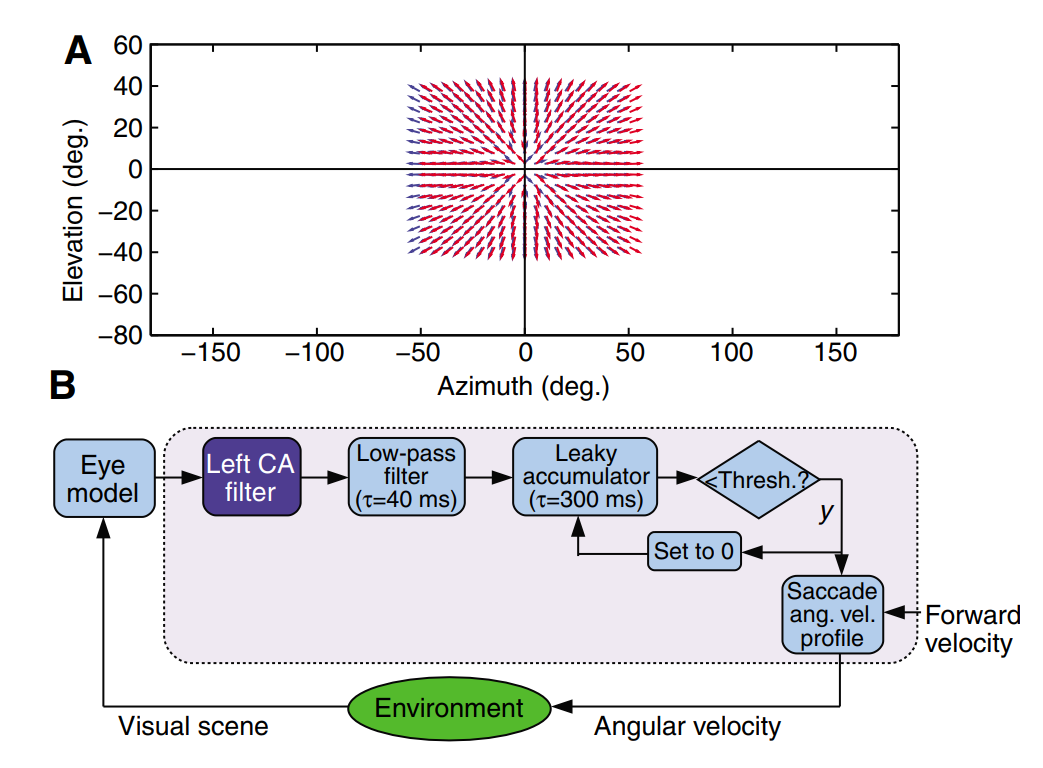
\includegraphics[width=0.9\textwidth]{Stewart2010CAModel}
  \caption{
    \label{fig:stewartca} The OF filter model: (Caption from \textit{Stewart et al.} Figure 7):
    Collision avoidance (CA). (A)The CA filters used in the
    model. Each covers ~105 deg. of azimuth but they are centred
    at $\pm 3$ deg. (elevation = 0 deg.). (B) Control diagram for collision
    avoidance. Only the half of the system that triggers rightward
    saccades is shown for clarity; the other half has an identical
    configuration. The dark blue box represents the blue wide-field
    filter in A. The reset operation also applies to the other half of
    the system, i.e. a saccade in one direction sets both
    accumulators to 0. Thresh., threshold; ang. vel., angular velocity.
  }
 
\end{figure}

\subsection{ The Mushroom Body for Visual Navigation } \label{MBBackground}
The Mushroom Body neuropils are structures present in the brains of insects though they are
largest in the brains of hymenoptera. They are known to play a critical role in olfactory
learning, and have been thought to play a role in visual memory in hymenoptera since 1982
at the latest\cite{Mobbs1982}. In 2016 a Mushroom Body circuit was proposed by \textit{Ardin et al.}
to allow emulation of the structure in a simulated desert ant \cite{Ardin2016}. The simulated
ant's view is taken from 1cm above the ground and has a field of view of $296^{\circ}$ azimuth
by $76^{\circ}$ elevation. A ratio of $4^{\circ}/pixel$ is used to give a $19\times74$ pixel image.
This image is then downsampled to 10$\times$36 pixels to give a realistic resolution for ant vision.
A $1\times360$ vector is used for further processing.
\newline

The generalised MB circuit is a three layer neural network: The first layer consists of a set of
visual Projection Neurons (vPNs), these connect to the second layer of standard artificial neurons
referred to as Kenyon Cells (KCs), and finally these KCs connect to a set of Extrinsic Neurons (ENs).
\newline

The model by \textit{Ardin et al.} (shown in Figure \ref{fig:ardinmb}) consisted of 350 vPNs
(one for each pixel in the downsampled image). In the second layer we have 20,000 KCs each of
which receives input from 10 randomly selected vPNs; each KC requires coincident input from multiple
vPNs to fire. Every KC is then connected to a single EN which sums the number of KCs which are
activated by the input image. The network is trained by providing a reward signal at regular
intervals. If KC activation coincides with a reward signal, the connection strength to the EN is
greatly reduced. The single EN simply gives a familiarity measure for the image seen. The agent
decides on its next action by scanning to find the direction of greatest familiarity.
\newline

\begin{figure}
  \centering
  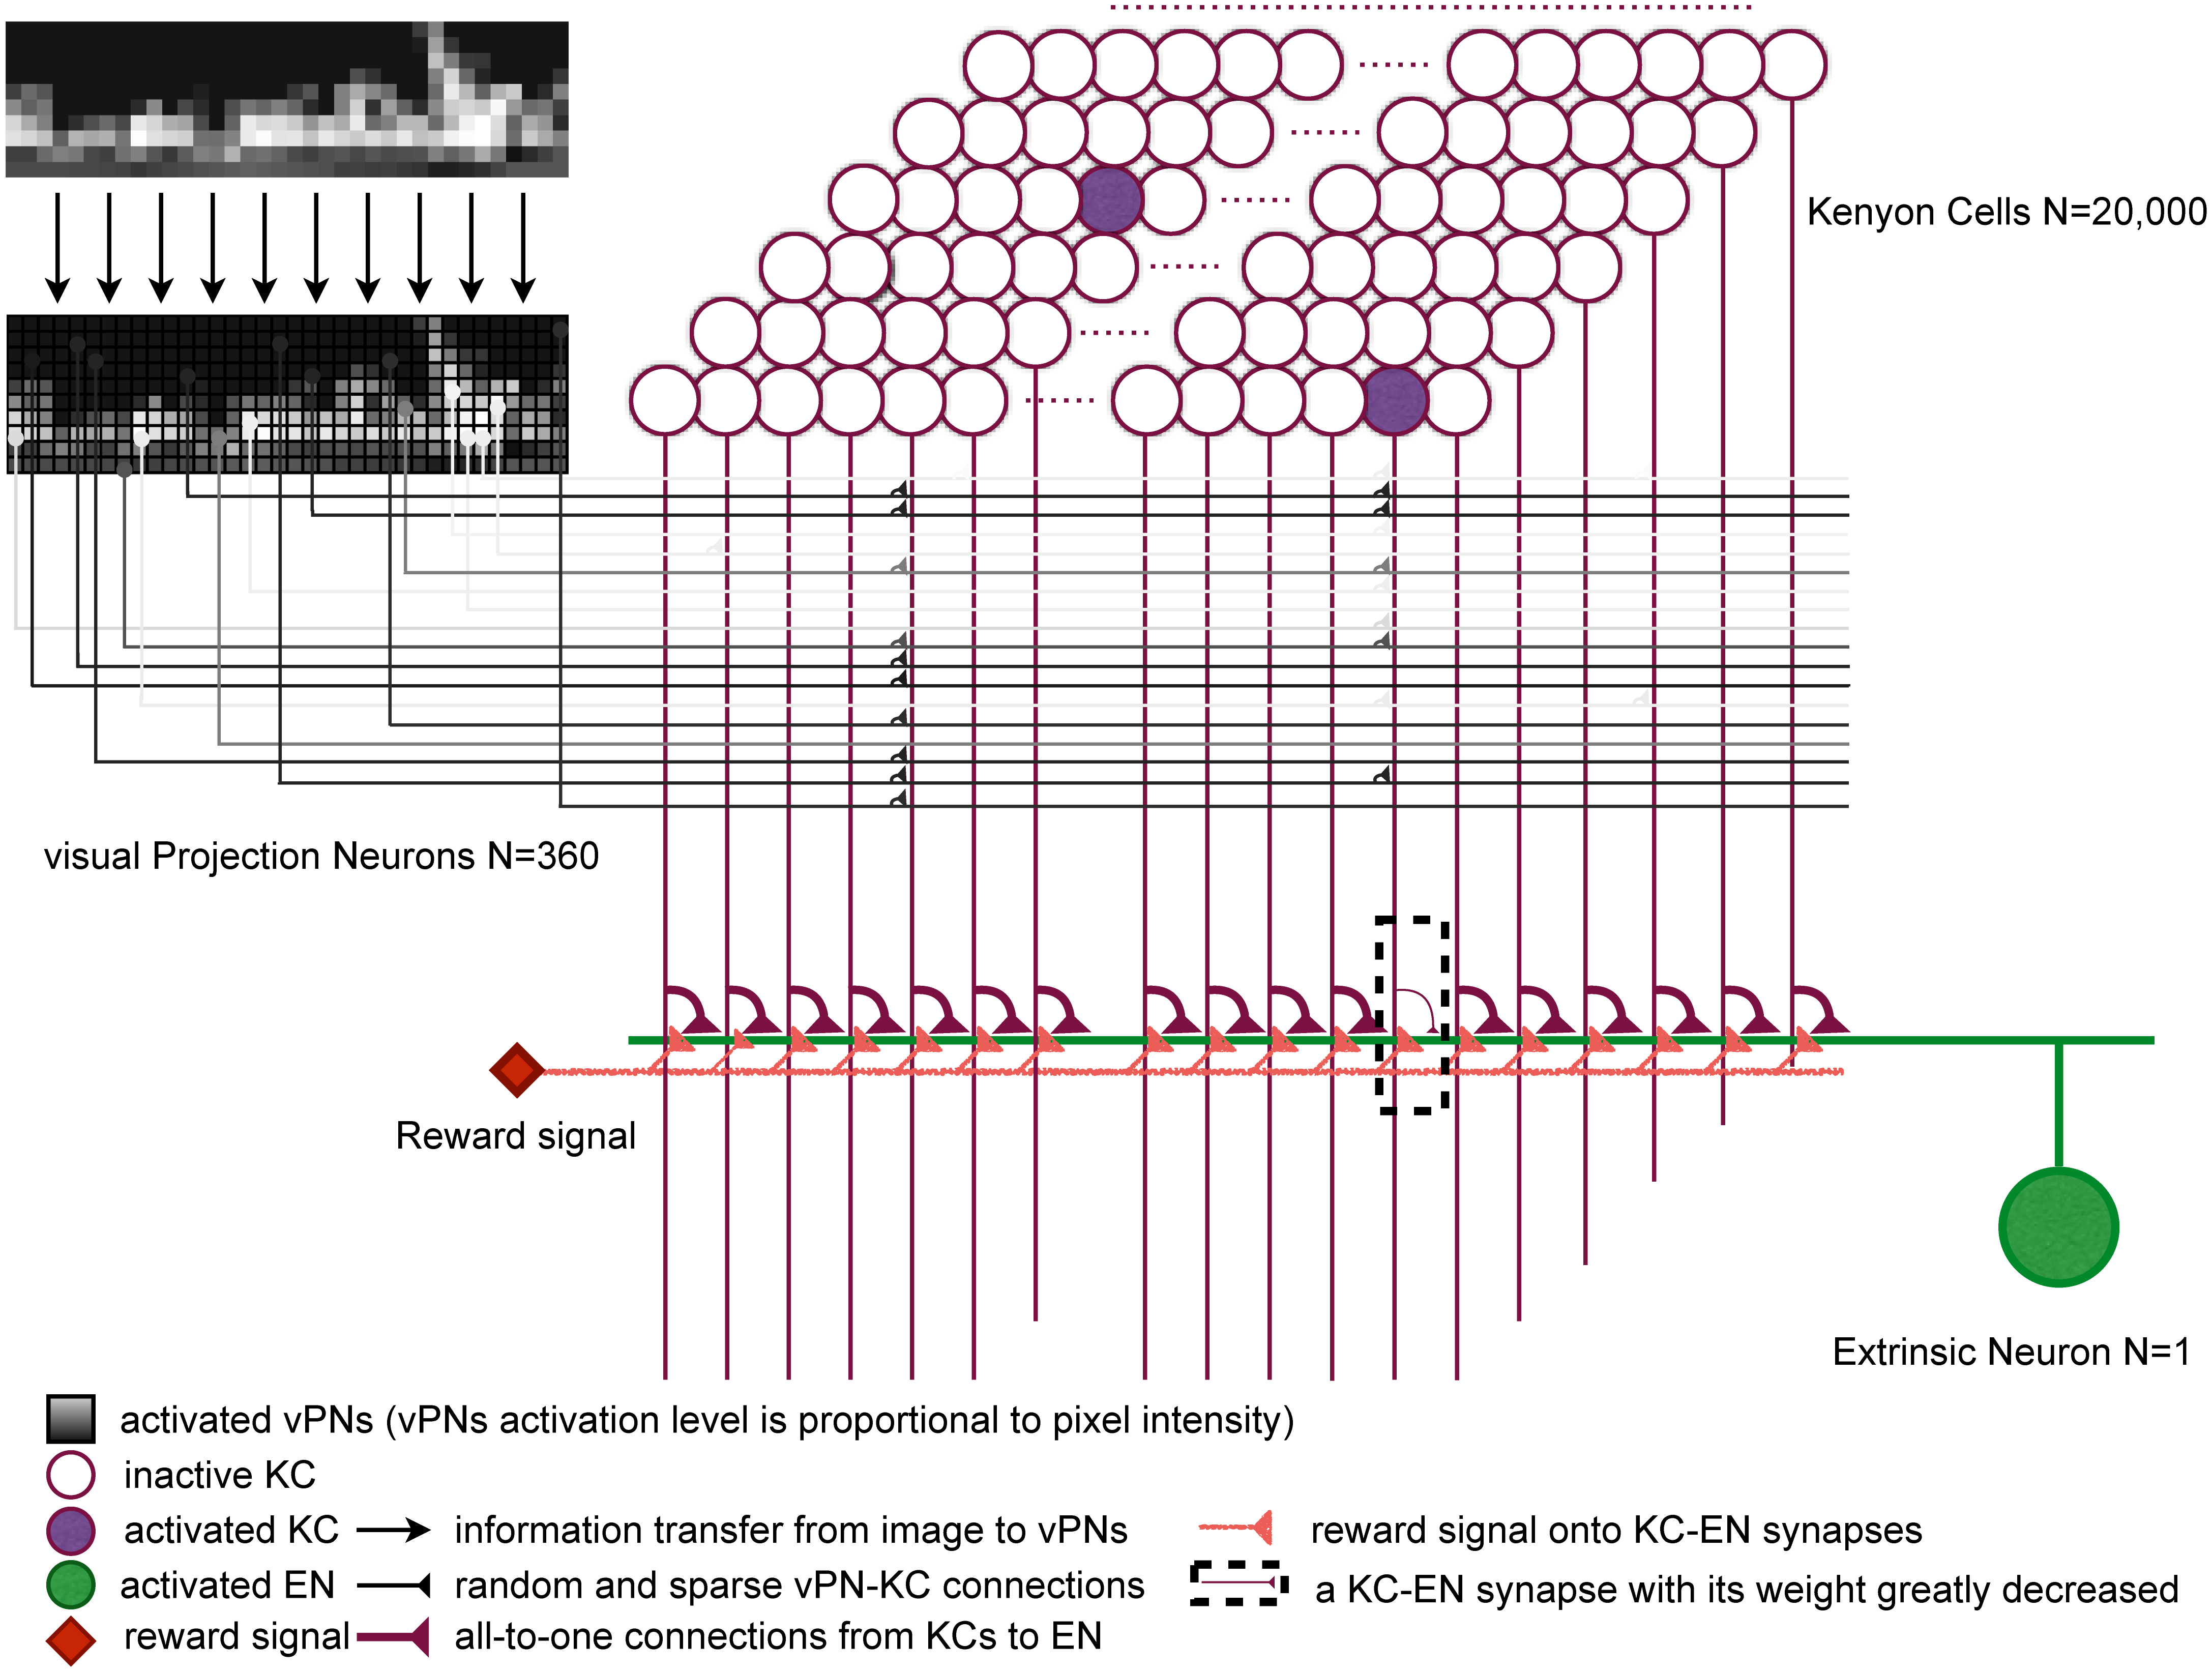
\includegraphics[width=0.9\textwidth]{Ardin2010MBModel}
  \caption{
    \label{fig:ardinmb} The Mushroom Body circuit: (Caption from \textit{Ardin et al.} Figure 2):
    Images (see Fig 1) activate the visual projection neurons (vPNs). Each Kenyon cell (KC) receives
    input from 10 (random) vPNs and exceeds firing threshold only for coincident activation from
    several vPNs, thus images are encoded as a sparse pattern of KC activation. All KCs converge on
    a single extrinsic neuron (EN) and if activation coincides with a reward signal, the connection
    strength is decreased. After training the EN output to previously rewarded (familiar) images is
    few or no spikes.
  }
\end{figure}

This version of the MB circuit has demonstrated the capacity to learn scene information, as well
as recapitulate routes by using the scanning technique \cite{Ardin2016}. In 2016, \textit{Eberding}
implemented the Willshaw Network (WN) on AntBot, which resembles the Mushroom Body neuropils; he
demonstrated that the network allowed the agent to perform visual navigation through a sparse testing
environment\cite{Eberding2016}. The agent navigates by scanning, computing unfamiliarity, and finally
choosing the direction of minimum unfamiliarity. In order to save on computational resources, the
KCs are binary rather than spiking (we hope to explore a spiking model later). While this does
generate a correct route, it is not as continuous as those performed by real ants.
\newline

In 2017, \textit{Zhang} implemented a route following strategy originally proposed by
\textit{Koszhabashev and Mangan} which employed klinokinesis in place of scanning. Klinokinesis
is one of two main forms of kinesis - the movement of an organism in response to stimulus - in which
the turning rate is proportional to stimulus intensity. In \cite{Zhang2017}, the
stimulus is given by the unfamiliarity metric generated by the MB model. The step size between each
turning point as well as the turning angle depends on the unfamiliarity of the current view. The same
algorithm from \cite{Kodzhabashev2015} is used to perform klinokinesis on the robot.
\newline

A separate model, also implemented by \textit{Zhang}, added seven extrinsic neurons. Each EN is then
used to represent one of eight directions relative to the robot's current heading; if we take 0$^\circ$
to be the robot's forward direction then the other seven directions correspond to $+45^\circ$,
$+90^\circ$, $+135^\circ$, $\pm180^\circ$, $-135^\circ$, $-90^\circ$, and $-45^\circ$. This model was implemented as a way of
combining the MB model for visual navigation and the CX model for path integration. While, path
integration and the CX model are not explored in this project, the model is still worth discussing,
as it may still be used to encode a desired response to specific stimuli.

%Should the Klinokinesis Algorithm be given here?

\newpage

%%%%%%%%%%%%%%%%%%%%%%%%%%%%%%%%%%%%%%%%%%%%%%%%%%%%%%%%%%%%%%%%%%%%%%%%%%%%%%% PLATFORM
\section{ Platform } \label{sec:platform}
In order to test the hypothesised models for ant navigation we use a simple robot autonomous - AntBot.
AntBot was originally developed by \textit{Eberding} in 2016; here we will discuss his design and
implementation, upon which we develop our algorithms.

\subsection{ Hardware }
AntBot's predecessor, Roboant, was originally designed by \textit{Kodzhabashev} \cite{Kodzhabashev2014}
as a compact Android robot. The robot required only four components: A sufficiently powerful Android
phone (A Google Nexus 5 was used) as the brain, the Zumo Robot shield by Pololu as the chassis,
an Arduino microcontroller to allow them to communicate, and finally a 360$^{\circ}$ camera attachment.
AntBot uses the same basic structure, however, a Dangu 5 Rover chassis is used as the base, and
therefore an alternate motor controller board had to be used.
\newline

The Android phone was chosen as the control module for the robot for a number of reasons. Firstly,
the hardware; a modern smartphone allows a compact, powerful platform on which to build the
software system as well as providing built in sensory systems and the libraries to use them (e.g. the
camera). The Google Nexus 5 is more than capable of running image processing software, analysing
optical flow patterns, and simulating the required artifical neural networks required for this project.
Using an Android platform also allows for modular software design (See section \ref{subsubsec:droid}).
In order to mimic the near 360$^{\circ}$ field of view (FOV) given by the ant's compound eyes, we use a
panoramic lense (the Kogeto Dot), which uses a convex mirror to give a full 360$^{\circ}$ FOV. This
lense is attached to the front camera and requires some pre-processing to retrieve the desired
$360\times40$ image. As with Roboant, the Android phone is connected to an Arduino using a serial
interface. Commands are sent from the phone to the Arduino which then executes the relevant commands
on the motor board to provide motion control.

\begin{figure}[t!]
  \centering
  \begin{minipage}[t!]{0.45\textwidth}
    \centering
    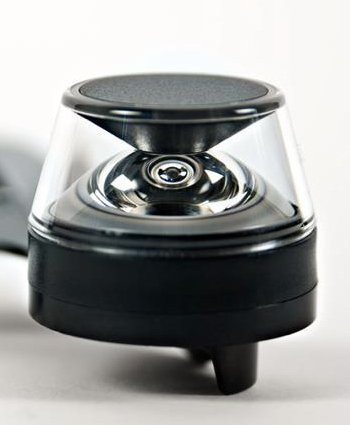
\includegraphics[width=0.9\textwidth]{KogetoDot}
    \caption{The Kogeto Dot 360$^\circ$ panoramic lens.}
  \end{minipage}
  \hfill
  \begin{minipage}[t!]{0.45\textwidth}
    \centering
    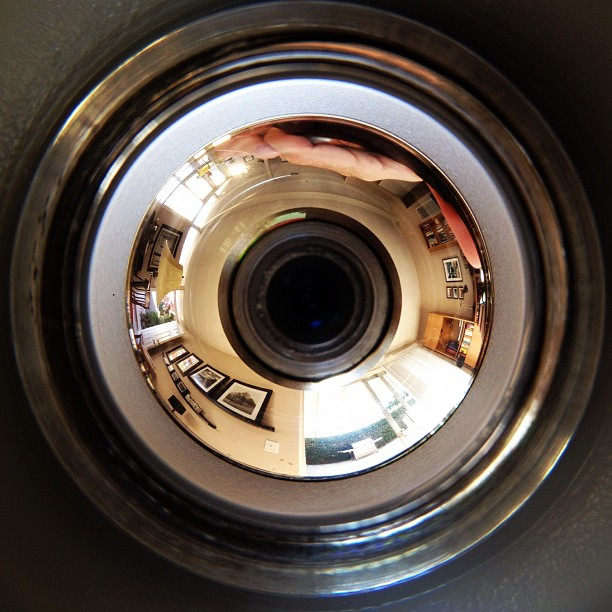
\includegraphics[width=0.9\textwidth]{PanoramicView}
    \caption{A sample of the view given by the lense pre-processing.}
  \end{minipage}

\end{figure}

\subsection{ Software }
\subsubsection{ Android } \label{subsubsec:droid}
The architecture of the Anrdoid operating system is such that applications can (subject to certain
constraints) run in parallel while broadcasting important information to one another. This allows
for a modular, ROS-like\footnote{Robot Operating System - ROS: http://www.ros.org/}
system in which we can have a dedicated application for each navigational subsystem employed by AntBot.
\newline

In this fashion, \textit{Eberding} implemented an Android Application Network (AAN) consisting of
five applications:
\newline

\begin{enumerate}
\item{
    The \textit{AntEye} application - This application is the main application in the network and
    provides the user interface, along with all camera interaction and visual processing. To summarise;
    the visual processing system takes the 360$^{\circ}$ panoramic image from the camera, extracts
    the blue channel information, crops out the ring which contains the actual image and reshapes
    this into a $360\times40px$ image, and finally downsamples this to a $90\times10px$ image. This
    final image is then used by any application which requires visual information.
  }

\item{
    The \textit{Path Integration} application - This application is responsible for performing all
    tasks related to Path Integration (PI). PI is the process of computing displacement
    based on a series of consecutive moves. In \textit{Eberding's} original implementation this
    application did not perform PI, but was instead used as a utility application to record orientation
    and distance travelled. \textit{Scimeca} extended this application to implement PI, using both a
    mathematical and neural approach.
  }

\item{
    The \textit{Visual Navigation} application - Similar to the PI application, the VN application
    houses the necessary components for performing visual navigation tasks. \textit{Eberding}
    implemented both the Willshaw (Mushroom Body) network, and also a Perfect Memory (PM) module both
    of which were extended by \textit{Zhang}. There also exists a super-class for visual navigation
    algorithms.
    }

\item{
    The \textit{Combiner} application - This application is used to combine the output from the

    VN and PI applications in order to compute what action the robot should take. This application
    governs the movement of the robot based on the two primary navigational systems.
  }

\item{
    The \textit{Serial Communications} application - This application governs all communication from
    the Android phone to the Arduino and server-interface. Android forbids multiple applications from
    using a single serial or Wifi port, so this application was developed as an intermediary to allow
    the other applications in the network to communicate through a single application.
    }
\end{enumerate}


\textit{Eberding's} implementation included a server interface which was used to control the robot
remotely
using the phone's Wifi hotspot and Serial Communicatin App, however, this interface has not been used
since the original implementation. For more information, please see \cite{Eberding2016}. It should
also be noted that, due to work conducted during previous iterations of this project, it may not
be possible to follow this exact structure.


\subsubsection{Arduino}
The Arduino software can be split into two sections: the \textit{parser} and the \textit{executioner}.
The parser will receive commands from the serial port and convert them into a series of movement
commands. These movement commands are then sent to the motor board by the executioner. Encoder
information may be gathered by the Arduino and sent back to the phone for processing.
For this project,
the Arduino code has not been modified. We only required the use of two commands for this project;
\textit{go}, which allows the robot to move indefinitely at a set speed, and \textit{turn}, which
allows the robot to turn to a desired (relative) angle. The \textit{go} command also allows the
operator to specify a speed for the left and right sides allowing the robot to move in smooth arcs.
A full list of commands can be seen in Table \ref{tab:commands}.

\begin{center}
  \begin{table}
    \begin{tabular}{ | l | l | p{7cm} | }

      \hline
      \textbf{Command} & \textbf{Message} & \textbf{Action} \\ \hline
      
      Heartbeat & x \textit{seconds} n &   Feedback sent to verify a stable connection between the
                                           phone and the Arduino. A signal is sent every second with a
                                           timestamp and checked. \\ \hline

      Move & t 0 \textit{distance} n & Travel a set distance in metres. \\  \hline
      Turn & t 0 \textit{angle} m 0 n & Turn a set angle (in degrees). \\ \hline
      Turn and Move & t \textit{angle} m \textit{distance} n & Turn by a specified angle then move the
                                                               specified distance. \\ \hline
      Turn left & \textit{l} & Turn left indefinitely. \\ \hline
      Turn right & \textit{r} & Turn right indefinitely. \\ \hline
      Halt & \textit{h} & Stop any command in progress and stop the robot. \\ \hline
      Go & g \textit{leftSpeed} \textit{rightSpeed} n & Move indefinitely with specified left and
                                                        right speeds. \\ \hline
                               
      
      \hline
      


      
    \end{tabular}
    \caption{The available commands on the Arduino and the messages sent to invoke them. Those
      values which are changeable are shown in italics. The \textit{go} command was added by
      \textit{Scimeca}. This table was adapted from \cite{Eberding2016, Scimeca2017}.
    }
    \label{tab:commands}
  \end{table}
\end{center}

Previous works have mentioned a message of the format \textit{e e1 e2 e3 e4} n. This message was used
to send wheel encoder information from the Arduino to the phone, however, this message was only sent
during the execution of a particular function and it has since been removed from the Arduino code.
There are currently no utilities available to retrieve and reset encoder values on-demand from the
phone, though this should not be difficult to implement.

\newpage
%%%%%%%%%%%%%%%%%%%%%%%%%%%%%%%%%%%%%%%%%%%%%%%%%%%%%%%%%%%%%%%%%%%%%%%%%%%%%%% METHODS
\section{ Methods } \label{sec:methods}
\textit{Included for skeleton purposes.}

\newpage

\section{ Results and Evalutation } \label{sec:results}
\textit{Included for skeleton purposes.}

\newpage

\section{ Discussion } \label{sec:discussion}
\textit{Included for skeleton purposes.} 

\newpage

\bibliographystyle{plain}
\bibliography{working}

\end{document}




